\documentclass[1p]{elsarticle_modified}
%\bibliographystyle{elsarticle-num}

%\usepackage[colorlinks]{hyperref}
%\usepackage{abbrmath_seonhwa} %\Abb, \Ascr, \Acal ,\Abf, \Afrak
\usepackage{amsfonts}
\usepackage{amssymb}
\usepackage{amsmath}
\usepackage{amsthm}
\usepackage{scalefnt}
\usepackage{amsbsy}
\usepackage{kotex}
\usepackage{caption}
\usepackage{subfig}
\usepackage{color}
\usepackage{graphicx}
\usepackage{xcolor} %% white, black, red, green, blue, cyan, magenta, yellow
\usepackage{float}
\usepackage{setspace}
\usepackage{hyperref}

\usepackage{tikz}
\usetikzlibrary{arrows}

\usepackage{multirow}
\usepackage{array} % fixed length table
\usepackage{hhline}

%%%%%%%%%%%%%%%%%%%%%
\makeatletter
\renewcommand*\env@matrix[1][\arraystretch]{%
	\edef\arraystretch{#1}%
	\hskip -\arraycolsep
	\let\@ifnextchar\new@ifnextchar
	\array{*\c@MaxMatrixCols c}}
\makeatother %https://tex.stackexchange.com/questions/14071/how-can-i-increase-the-line-spacing-in-a-matrix
%%%%%%%%%%%%%%%

\usepackage[normalem]{ulem}

\newcommand{\msout}[1]{\ifmmode\text{\sout{\ensuremath{#1}}}\else\sout{#1}\fi}
%SOURCE: \msout is \stkout macro in https://tex.stackexchange.com/questions/20609/strikeout-in-math-mode

\newcommand{\cancel}[1]{
	\ifmmode
	{\color{red}\msout{#1}}
	\else
	{\color{red}\sout{#1}}
	\fi
}

\newcommand{\add}[1]{
	{\color{blue}\uwave{#1}}
}

\newcommand{\replace}[2]{
	\ifmmode
	{\color{red}\msout{#1}}{\color{blue}\uwave{#2}}
	\else
	{\color{red}\sout{#1}}{\color{blue}\uwave{#2}}
	\fi
}

\newcommand{\Sol}{\mathcal{S}} %segment
\newcommand{\D}{D} %diagram
\newcommand{\A}{\mathcal{A}} %arc


%%%%%%%%%%%%%%%%%%%%%%%%%%%%%5 test

\def\sl{\operatorname{\textup{SL}}(2,\Cbb)}
\def\psl{\operatorname{\textup{PSL}}(2,\Cbb)}
\def\quan{\mkern 1mu \triangleright \mkern 1mu}

\theoremstyle{definition}
\newtheorem{thm}{Theorem}[section]
\newtheorem{prop}[thm]{Proposition}
\newtheorem{lem}[thm]{Lemma}
\newtheorem{ques}[thm]{Question}
\newtheorem{cor}[thm]{Corollary}
\newtheorem{defn}[thm]{Definition}
\newtheorem{exam}[thm]{Example}
\newtheorem{rmk}[thm]{Remark}
\newtheorem{alg}[thm]{Algorithm}

\newcommand{\I}{\sqrt{-1}}
\begin{document}

%\begin{frontmatter}
%
%\title{Boundary parabolic representations of knots up to 8 crossings}
%
%%% Group authors per affiliation:
%\author{Yunhi Cho} 
%\address{Department of Mathematics, University of Seoul, Seoul, Korea}
%\ead{yhcho@uos.ac.kr}
%
%
%\author{Seonhwa Kim} %\fnref{s_kim}}
%\address{Center for Geometry and Physics, Institute for Basic Science, Pohang, 37673, Korea}
%\ead{ryeona17@ibs.re.kr}
%
%\author{Hyuk Kim}
%\address{Department of Mathematical Sciences, Seoul National University, Seoul 08826, Korea}
%\ead{hyukkim@snu.ac.kr}
%
%\author{Seokbeom Yoon}
%\address{Department of Mathematical Sciences, Seoul National University, Seoul, 08826,  Korea}
%\ead{sbyoon15@snu.ac.kr}
%
%\begin{abstract}
%We find all boundary parabolic representation of knots up to 8 crossings.
%
%\end{abstract}
%\begin{keyword}
%    \MSC[2010] 57M25 
%\end{keyword}
%
%\end{frontmatter}

%\linenumbers
%\tableofcontents
%
\newcommand\colored[1]{\textcolor{white}{\rule[-0.35ex]{0.8em}{1.4ex}}\kern-0.8em\color{red} #1}%
%\newcommand\colored[1]{\textcolor{white}{ #1}\kern-2.17ex	\textcolor{white}{ #1}\kern-1.81ex	\textcolor{white}{ #1}\kern-2.15ex\color{red}#1	}

{\Large $\underline{12n_{0697}~(K12n_{0697})}$}

\setlength{\tabcolsep}{10pt}
\renewcommand{\arraystretch}{1.6}
\vspace{1cm}\begin{tabular}{m{100pt}>{\centering\arraybackslash}m{274pt}}
\multirow{5}{120pt}{
	\centering
	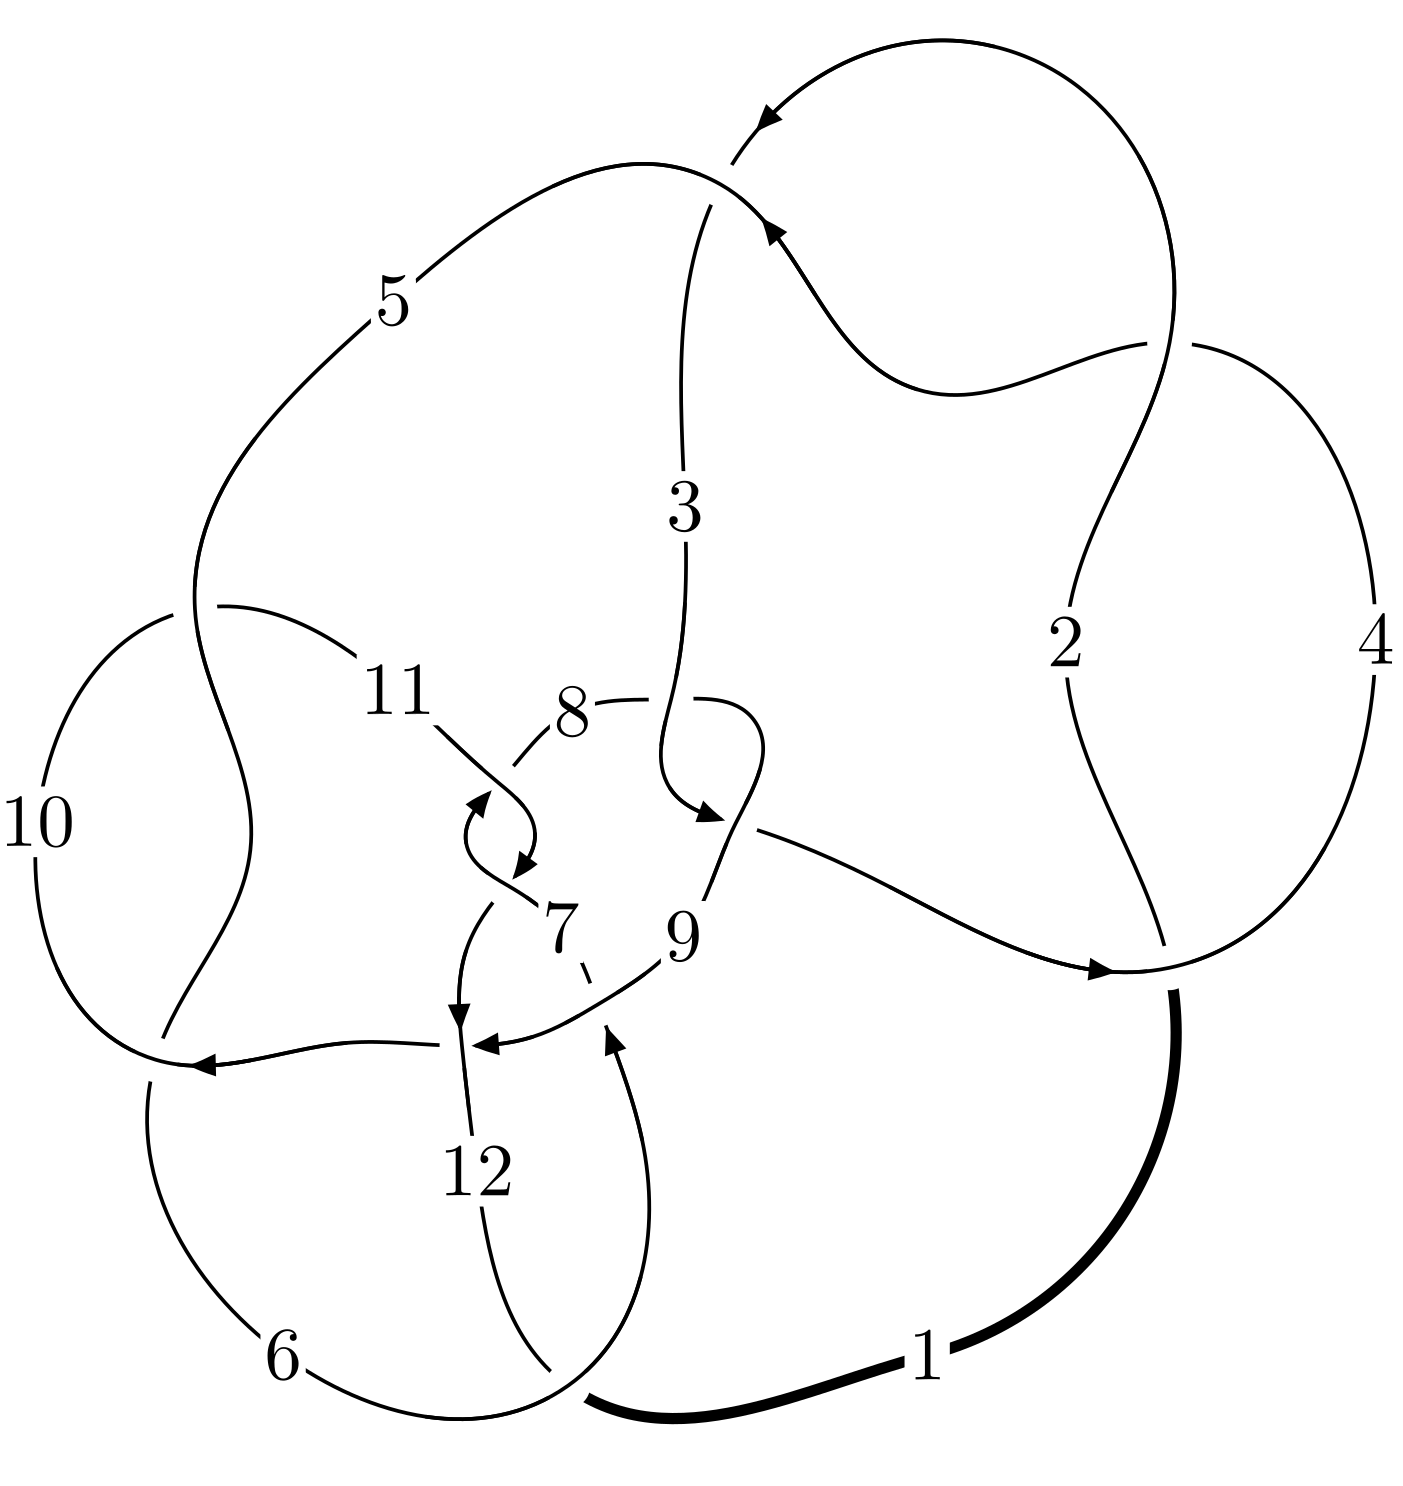
\includegraphics[width=112pt]{../../../GIT/diagram.site/Diagrams/png/2786_12n_0697.png}\\
\ \ \ A knot diagram\footnotemark}&
\allowdisplaybreaks
\textbf{Linearized knot diagam} \\
\cline{2-2}
 &
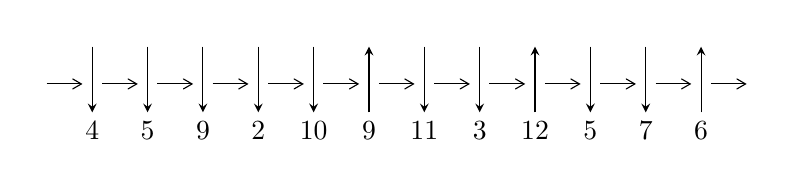
\begin{tikzpicture}[x=20pt, y=17pt]
	% nodes
	\node (C0) at (0, 0) {};
	\node (C1) at (1, 0) {};
	\node (C1U) at (1, +1) {};
	\node (C1D) at (1, -1) {4};

	\node (C2) at (2, 0) {};
	\node (C2U) at (2, +1) {};
	\node (C2D) at (2, -1) {5};

	\node (C3) at (3, 0) {};
	\node (C3U) at (3, +1) {};
	\node (C3D) at (3, -1) {9};

	\node (C4) at (4, 0) {};
	\node (C4U) at (4, +1) {};
	\node (C4D) at (4, -1) {2};

	\node (C5) at (5, 0) {};
	\node (C5U) at (5, +1) {};
	\node (C5D) at (5, -1) {10};

	\node (C6) at (6, 0) {};
	\node (C6U) at (6, +1) {};
	\node (C6D) at (6, -1) {9};

	\node (C7) at (7, 0) {};
	\node (C7U) at (7, +1) {};
	\node (C7D) at (7, -1) {11};

	\node (C8) at (8, 0) {};
	\node (C8U) at (8, +1) {};
	\node (C8D) at (8, -1) {3};

	\node (C9) at (9, 0) {};
	\node (C9U) at (9, +1) {};
	\node (C9D) at (9, -1) {12};

	\node (C10) at (10, 0) {};
	\node (C10U) at (10, +1) {};
	\node (C10D) at (10, -1) {5};

	\node (C11) at (11, 0) {};
	\node (C11U) at (11, +1) {};
	\node (C11D) at (11, -1) {7};

	\node (C12) at (12, 0) {};
	\node (C12U) at (12, +1) {};
	\node (C12D) at (12, -1) {6};
	\node (C13) at (13, 0) {};

	% arrows
	\draw[->,>={angle 60}]
	(C0) edge (C1) (C1) edge (C2) (C2) edge (C3) (C3) edge (C4) (C4) edge (C5) (C5) edge (C6) (C6) edge (C7) (C7) edge (C8) (C8) edge (C9) (C9) edge (C10) (C10) edge (C11) (C11) edge (C12) (C12) edge (C13) ;	\draw[->,>=stealth]
	(C1U) edge (C1D) (C2U) edge (C2D) (C3U) edge (C3D) (C4U) edge (C4D) (C5U) edge (C5D) (C6D) edge (C6U) (C7U) edge (C7D) (C8U) edge (C8D) (C9D) edge (C9U) (C10U) edge (C10D) (C11U) edge (C11D) (C12D) edge (C12U) ;
	\end{tikzpicture} \\
\hhline{~~} \\& 
\textbf{Solving Sequence} \\ \cline{2-2} 
 &
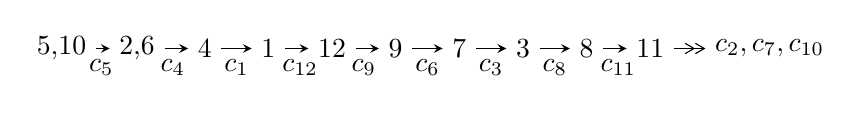
\begin{tikzpicture}[x=23pt, y=7pt]
	% node
	\node (A0) at (-1/8, 0) {5,10};
	\node (A1) at (17/16, 0) {2,6};
	\node (A2) at (17/8, 0) {4};
	\node (A3) at (25/8, 0) {1};
	\node (A4) at (33/8, 0) {12};
	\node (A5) at (41/8, 0) {9};
	\node (A6) at (49/8, 0) {7};
	\node (A7) at (57/8, 0) {3};
	\node (A8) at (65/8, 0) {8};
	\node (A9) at (73/8, 0) {11};
	\node (C1) at (1/2, -1) {$c_{5}$};
	\node (C2) at (13/8, -1) {$c_{4}$};
	\node (C3) at (21/8, -1) {$c_{1}$};
	\node (C4) at (29/8, -1) {$c_{12}$};
	\node (C5) at (37/8, -1) {$c_{9}$};
	\node (C6) at (45/8, -1) {$c_{6}$};
	\node (C7) at (53/8, -1) {$c_{3}$};
	\node (C8) at (61/8, -1) {$c_{8}$};
	\node (C9) at (69/8, -1) {$c_{11}$};
	\node (A10) at (11, 0) {$c_{2},c_{7},c_{10}$};

	% edge
	\draw[->,>=stealth]	
	(A0) edge (A1) (A1) edge (A2) (A2) edge (A3) (A3) edge (A4) (A4) edge (A5) (A5) edge (A6) (A6) edge (A7) (A7) edge (A8) (A8) edge (A9) ;
	\draw[->>,>={angle 60}]	
	(A9) edge (A10);
\end{tikzpicture} \\ 

\end{tabular} \\

\footnotetext{
The image of knot diagram is generated by the software ``\textbf{Draw programme}" developed by Andrew Bartholomew(\url{http://www.layer8.co.uk/maths/draw/index.htm\#Running-draw}), where we modified some parts for our purpose(\url{https://github.com/CATsTAILs/LinksPainter}).
}\phantom \\ \newline 
\centering \textbf{Ideals for irreducible components\footnotemark of $X_{\text{par}}$} 
 
\begin{align*}
I^u_{1}&=\langle 
-3.62104\times10^{19} u^{20}+1.26138\times10^{19} u^{19}+\cdots+4.08630\times10^{20} b+4.01944\times10^{20},\\
\phantom{I^u_{1}}&\phantom{= \langle  }-1.37856\times10^{21} u^{20}-8.38333\times10^{20} u^{19}+\cdots+5.72082\times10^{21} a-9.06403\times10^{21},\;u^{21}-3 u^{19}+\cdots- u+1\rangle \\
I^u_{2}&=\langle 
b+1,\;- u^3- u^2+2 a- u+1,\;u^4+u^2- u+1\rangle \\
I^u_{3}&=\langle 
-2 u^{11}+u^{10}-5 u^9+10 u^8+5 u^7+22 u^6+17 u^5+16 u^4+13 u^3+9 u^2+b+6 u+2,\\
\phantom{I^u_{3}}&\phantom{= \langle  }-4 u^{12}+5 u^{11}-12 u^{10}+28 u^9-6 u^8+41 u^7+12 u^5-5 u^4-5 u^3-9 u^2+a-6 u-5,\\
\phantom{I^u_{3}}&\phantom{= \langle  }u^{13}+3 u^{11}-4 u^{10}-3 u^9-16 u^8-16 u^7-22 u^6-18 u^5-16 u^4-11 u^3-7 u^2-3 u-1\rangle \\
I^u_{4}&=\langle 
b+1,\;u^5+2 u^3+a+u+1,\;u^6+u^5+2 u^4+2 u^3+2 u^2+2 u+1\rangle \\
I^u_{5}&=\langle 
-31240024 u^{11}-108045960 u^{10}+\cdots+16035124397 b+4787221942,\\
\phantom{I^u_{5}}&\phantom{= \langle  }-2479067476388 u^{11}-7672762434312 u^{10}+\cdots+189470000096321 a-300611169358247,\\
\phantom{I^u_{5}}&\phantom{= \langle  }u^{12}+2 u^{11}- u^{10}+24 u^8+24 u^7-42 u^6+142 u^5-296 u^4+168 u^3-248 u^2+192 u-79\rangle \\
\\
\end{align*}
\raggedright * 5 irreducible components of $\dim_{\mathbb{C}}=0$, with total 56 representations.\\
\footnotetext{All coefficients of polynomials are rational numbers. But the coefficients are sometimes approximated in decimal forms when there is not enough margin.}
\newpage
\renewcommand{\arraystretch}{1}
\centering \section*{I. $I^u_{1}= \langle -3.62\times10^{19} u^{20}+1.26\times10^{19} u^{19}+\cdots+4.09\times10^{20} b+4.02\times10^{20},\;-1.38\times10^{21} u^{20}-8.38\times10^{20} u^{19}+\cdots+5.72\times10^{21} a-9.06\times10^{21},\;u^{21}-3 u^{19}+\cdots- u+1 \rangle$}
\flushleft \textbf{(i) Arc colorings}\\
\begin{tabular}{m{7pt} m{180pt} m{7pt} m{180pt} }
\flushright $a_{5}=$&$\begin{pmatrix}1\\0\end{pmatrix}$ \\
\flushright $a_{10}=$&$\begin{pmatrix}0\\u\end{pmatrix}$ \\
\flushright $a_{2}=$&$\begin{pmatrix}0.240973 u^{20}+0.146541 u^{19}+\cdots+0.630949 u+1.58439\\0.0886140 u^{20}-0.0308685 u^{19}+\cdots+0.687354 u-0.983638\end{pmatrix}$ \\
\flushright $a_{6}=$&$\begin{pmatrix}1\\u^2\end{pmatrix}$ \\
\flushright $a_{4}=$&$\begin{pmatrix}0.569574 u^{20}+0.221291 u^{19}+\cdots-0.866797 u+0.435171\\-0.376569 u^{20}-0.348821 u^{19}+\cdots+2.18805 u+0.671636\end{pmatrix}$ \\
\flushright $a_{1}=$&$\begin{pmatrix}-0.0422288 u^{20}-0.00485208 u^{19}+\cdots-0.760876 u+0.127899\\-0.411664 u^{20}-0.138444 u^{19}+\cdots+3.07667 u+1.14698\end{pmatrix}$ \\
\flushright $a_{12}=$&$\begin{pmatrix}0.367023 u^{20}+0.127899 u^{19}+\cdots-3.80016 u-1.01423\\-0.367023 u^{20}-0.127899 u^{19}+\cdots+2.80016 u+1.01423\end{pmatrix}$ \\
\flushright $a_{9}=$&$\begin{pmatrix}0.410427 u^{20}+0.0856689 u^{19}+\cdots-1.95365 u-1.18436\\-0.368198 u^{20}-0.0808168 u^{19}+\cdots+2.71453 u+1.05646\end{pmatrix}$ \\
\flushright $a_{7}=$&$\begin{pmatrix}-1.01423 u^{20}-0.367023 u^{19}+\cdots+4.62375 u+3.81439\\1.01423 u^{20}+0.367023 u^{19}+\cdots-4.62375 u-2.81439\end{pmatrix}$ \\
\flushright $a_{3}=$&$\begin{pmatrix}0.152359 u^{20}+0.177409 u^{19}+\cdots-0.0564046 u+2.56803\\0.0886140 u^{20}-0.0308685 u^{19}+\cdots+0.687354 u-0.983638\end{pmatrix}$ \\
\flushright $a_{8}=$&$\begin{pmatrix}1.01423 u^{20}+0.367023 u^{19}+\cdots-4.62375 u-3.81439\\-1.01423 u^{20}-0.367023 u^{19}+\cdots+4.62375 u+2.81439\end{pmatrix}$ \\
\flushright $a_{11}=$&$\begin{pmatrix}- u\\u\end{pmatrix}$\\&\end{tabular}
\flushleft \textbf{(ii) Obstruction class $= -1$}\\~\\
\flushleft \textbf{(iii) Cusp Shapes $= -\frac{41331710946122587570789}{11441642780167527166456} u^{20}-\frac{13713223367732965094891}{11441642780167527166456} u^{19}+\cdots+\frac{62252584059208509594863}{2860410695041881791614} u+\frac{24448772877532289945923}{5720821390083763583228}$}\\~\\
\newpage\renewcommand{\arraystretch}{1}
\flushleft \textbf{(iv) u-Polynomials at the component}\newline \\
\begin{tabular}{m{50pt}|m{274pt}}
Crossings & \hspace{64pt}u-Polynomials at each crossing \\
\hline $$\begin{aligned}c_{1},c_{2},c_{4}\end{aligned}$$&$\begin{aligned}
&u^{21}-5 u^{20}+\cdots-176 u+64
\end{aligned}$\\
\hline $$\begin{aligned}c_{3},c_{8}\end{aligned}$$&$\begin{aligned}
&u^{21}+u^{20}+\cdots+3328 u+1024
\end{aligned}$\\
\hline $$\begin{aligned}c_{5},c_{7},c_{10}\\c_{11}\end{aligned}$$&$\begin{aligned}
&u^{21}-3 u^{19}+\cdots- u+1
\end{aligned}$\\
\hline $$\begin{aligned}c_{6},c_{12}\end{aligned}$$&$\begin{aligned}
&u^{21}+u^{20}+\cdots+26 u^2+1
\end{aligned}$\\
\hline $$\begin{aligned}c_{9}\end{aligned}$$&$\begin{aligned}
&u^{21}+7 u^{20}+\cdots+32 u+4
\end{aligned}$\\
\hline
\end{tabular}\\~\\
\newpage\renewcommand{\arraystretch}{1}
\flushleft \textbf{(v) Riley Polynomials at the component}\newline \\
\begin{tabular}{m{50pt}|m{274pt}}
Crossings & \hspace{64pt}Riley Polynomials at each crossing \\
\hline $$\begin{aligned}c_{1},c_{2},c_{4}\end{aligned}$$&$\begin{aligned}
&y^{21}-25 y^{20}+\cdots+9472 y-4096
\end{aligned}$\\
\hline $$\begin{aligned}c_{3},c_{8}\end{aligned}$$&$\begin{aligned}
&y^{21}-27 y^{20}+\cdots-1769472 y-1048576
\end{aligned}$\\
\hline $$\begin{aligned}c_{5},c_{7},c_{10}\\c_{11}\end{aligned}$$&$\begin{aligned}
&y^{21}-6 y^{20}+\cdots+9 y-1
\end{aligned}$\\
\hline $$\begin{aligned}c_{6},c_{12}\end{aligned}$$&$\begin{aligned}
&y^{21}+13 y^{20}+\cdots-52 y-1
\end{aligned}$\\
\hline $$\begin{aligned}c_{9}\end{aligned}$$&$\begin{aligned}
&y^{21}-5 y^{20}+\cdots+440 y-16
\end{aligned}$\\
\hline
\end{tabular}\\~\\
\newpage\flushleft \textbf{(vi) Complex Volumes and Cusp Shapes}
$$\begin{array}{c|c|c}  
\text{Solutions to }I^u_{1}& \I (\text{vol} + \sqrt{-1}CS) & \text{Cusp shape}\\
 \hline 
\begin{aligned}
u &= -0.749636 + 0.488902 I \\
a &= \phantom{-}0.469897 + 0.044424 I \\
b &= \phantom{-}0.341636 + 0.425477 I\end{aligned}
 & -1.45186 + 0.85737 I & -6.38463 - 1.62097 I \\ \hline\begin{aligned}
u &= -0.749636 - 0.488902 I \\
a &= \phantom{-}0.469897 - 0.044424 I \\
b &= \phantom{-}0.341636 - 0.425477 I\end{aligned}
 & -1.45186 - 0.85737 I & -6.38463 + 1.62097 I \\ \hline\begin{aligned}
u &= -0.139166 + 0.781262 I \\
a &= -0.73889 + 1.22004 I \\
b &= \phantom{-}1.375930 - 0.218020 I\end{aligned}
 & -3.48621 + 5.01960 I & -12.50321 + 2.57874 I \\ \hline\begin{aligned}
u &= -0.139166 - 0.781262 I \\
a &= -0.73889 - 1.22004 I \\
b &= \phantom{-}1.375930 + 0.218020 I\end{aligned}
 & -3.48621 - 5.01960 I & -12.50321 - 2.57874 I \\ \hline\begin{aligned}
u &= -0.099594 + 0.653522 I \\
a &= \phantom{-}0.28465 - 1.42599 I \\
b &= -0.166654 + 0.606297 I\end{aligned}
 & \phantom{-}1.43705 + 2.05574 I & -1.84211 - 3.02644 I \\ \hline\begin{aligned}
u &= -0.099594 - 0.653522 I \\
a &= \phantom{-}0.28465 + 1.42599 I \\
b &= -0.166654 - 0.606297 I\end{aligned}
 & \phantom{-}1.43705 - 2.05574 I & -1.84211 + 3.02644 I \\ \hline\begin{aligned}
u &= \phantom{-}0.713665 + 1.142840 I \\
a &= \phantom{-}0.257213 - 0.050637 I \\
b &= \phantom{-}0.917606 - 0.416133 I\end{aligned}
 & \phantom{-}1.15190 - 6.95574 I & -3.07603 + 1.63596 I \\ \hline\begin{aligned}
u &= \phantom{-}0.713665 - 1.142840 I \\
a &= \phantom{-}0.257213 + 0.050637 I \\
b &= \phantom{-}0.917606 + 0.416133 I\end{aligned}
 & \phantom{-}1.15190 + 6.95574 I & -3.07603 - 1.63596 I \\ \hline\begin{aligned}
u &= \phantom{-}0.118860 + 0.511212 I \\
a &= \phantom{-}0.21443 + 2.11251 I \\
b &= -1.120560 - 0.176119 I\end{aligned}
 & -1.29818 - 0.86925 I & -5.22327 - 0.45664 I \\ \hline\begin{aligned}
u &= \phantom{-}0.118860 - 0.511212 I \\
a &= \phantom{-}0.21443 - 2.11251 I \\
b &= -1.120560 + 0.176119 I\end{aligned}
 & -1.29818 + 0.86925 I & -5.22327 + 0.45664 I\\
 \hline 
 \end{array}$$\newpage$$\begin{array}{c|c|c}  
\text{Solutions to }I^u_{1}& \I (\text{vol} + \sqrt{-1}CS) & \text{Cusp shape}\\
 \hline 
\begin{aligned}
u &= \phantom{-}0.396570 + 0.053595 I \\
a &= \phantom{-}0.127913 - 0.750550 I \\
b &= \phantom{-}0.872784 + 0.806219 I\end{aligned}
 & \phantom{-}4.27603 - 3.00281 I & -0.00709 - 9.01951 I \\ \hline\begin{aligned}
u &= \phantom{-}0.396570 - 0.053595 I \\
a &= \phantom{-}0.127913 + 0.750550 I \\
b &= \phantom{-}0.872784 - 0.806219 I\end{aligned}
 & \phantom{-}4.27603 + 3.00281 I & -0.00709 + 9.01951 I \\ \hline\begin{aligned}
u &= -0.322867\phantom{ +0.000000I} \\
a &= \phantom{-}1.20351\phantom{ +0.000000I} \\
b &= -0.565313\phantom{ +0.000000I}\end{aligned}
 & -0.896054\phantom{ +0.000000I} & -11.8310\phantom{ +0.000000I} \\ \hline\begin{aligned}
u &= \phantom{-}1.14110 + 1.36056 I \\
a &= \phantom{-}0.796386 - 0.921717 I \\
b &= \phantom{-}1.89575 + 0.52604 I\end{aligned}
 & -18.0940 - 7.3272 I & -7.63094 + 2.78873 I \\ \hline\begin{aligned}
u &= \phantom{-}1.14110 - 1.36056 I \\
a &= \phantom{-}0.796386 + 0.921717 I \\
b &= \phantom{-}1.89575 - 0.52604 I\end{aligned}
 & -18.0940 + 7.3272 I & -7.63094 - 2.78873 I \\ \hline\begin{aligned}
u &= \phantom{-}1.83772 + 0.22825 I \\
a &= -0.768356 + 0.189539 I \\
b &= -1.69775 - 1.08714 I\end{aligned}
 & -7.41133 + 0.52434 I & -8.70349 - 1.08333 I \\ \hline\begin{aligned}
u &= \phantom{-}1.83772 - 0.22825 I \\
a &= -0.768356 - 0.189539 I \\
b &= -1.69775 + 1.08714 I\end{aligned}
 & -7.41133 - 0.52434 I & -8.70349 + 1.08333 I \\ \hline\begin{aligned}
u &= -1.86654 + 0.63952 I \\
a &= -0.678604 - 0.317967 I \\
b &= -1.55087 + 1.33931 I\end{aligned}
 & -7.05646 + 5.93668 I & -8.04055 - 3.74874 I \\ \hline\begin{aligned}
u &= -1.86654 - 0.63952 I \\
a &= -0.678604 + 0.317967 I \\
b &= -1.55087 - 1.33931 I\end{aligned}
 & -7.05646 - 5.93668 I & -8.04055 + 3.74874 I \\ \hline\begin{aligned}
u &= -1.19154 + 1.65776 I \\
a &= \phantom{-}0.683607 + 0.829952 I \\
b &= \phantom{-}1.91479 - 0.63403 I\end{aligned}
 & -16.9669 + 14.7114 I & -6.79810 - 5.93574 I\\
 \hline 
 \end{array}$$\newpage$$\begin{array}{c|c|c}  
\text{Solutions to }I^u_{1}& \I (\text{vol} + \sqrt{-1}CS) & \text{Cusp shape}\\
 \hline 
\begin{aligned}
u &= -1.19154 - 1.65776 I \\
a &= \phantom{-}0.683607 - 0.829952 I \\
b &= \phantom{-}1.91479 + 0.63403 I\end{aligned}
 & -16.9669 - 14.7114 I & -6.79810 + 5.93574 I\\
 \hline 
 \end{array}$$\newpage\newpage\renewcommand{\arraystretch}{1}
\centering \section*{II. $I^u_{2}= \langle b+1,\;- u^3- u^2+2 a- u+1,\;u^4+u^2- u+1 \rangle$}
\flushleft \textbf{(i) Arc colorings}\\
\begin{tabular}{m{7pt} m{180pt} m{7pt} m{180pt} }
\flushright $a_{5}=$&$\begin{pmatrix}1\\0\end{pmatrix}$ \\
\flushright $a_{10}=$&$\begin{pmatrix}0\\u\end{pmatrix}$ \\
\flushright $a_{2}=$&$\begin{pmatrix}\frac{1}{2} u^3+\frac{1}{2} u^2+\frac{1}{2} u-\frac{1}{2}\\-1\end{pmatrix}$ \\
\flushright $a_{6}=$&$\begin{pmatrix}1\\u^2\end{pmatrix}$ \\
\flushright $a_{4}=$&$\begin{pmatrix}\frac{1}{2} u^3+\frac{1}{2} u^2+\frac{1}{2} u+\frac{1}{2}\\-1\end{pmatrix}$ \\
\flushright $a_{1}=$&$\begin{pmatrix}-1\\0\end{pmatrix}$ \\
\flushright $a_{12}=$&$\begin{pmatrix}- u^2-1\\u^2- u+1\end{pmatrix}$ \\
\flushright $a_{9}=$&$\begin{pmatrix}- u^3- u^2\\u^3+u^2+1\end{pmatrix}$ \\
\flushright $a_{7}=$&$\begin{pmatrix}- u^3\\u^3+1\end{pmatrix}$ \\
\flushright $a_{3}=$&$\begin{pmatrix}\frac{1}{2} u^3+\frac{1}{2} u^2+\frac{1}{2} u+\frac{1}{2}\\-1\end{pmatrix}$ \\
\flushright $a_{8}=$&$\begin{pmatrix}- u^3- u^2\\u^3+u^2+1\end{pmatrix}$ \\
\flushright $a_{11}=$&$\begin{pmatrix}- u\\u\end{pmatrix}$\\&\end{tabular}
\flushleft \textbf{(ii) Obstruction class $= 1$}\\~\\
\flushleft \textbf{(iii) Cusp Shapes $= \frac{19}{4} u^3+\frac{13}{2} u^2-\frac{5}{2} u-\frac{37}{4}$}\\~\\
\newpage\renewcommand{\arraystretch}{1}
\flushleft \textbf{(iv) u-Polynomials at the component}\newline \\
\begin{tabular}{m{50pt}|m{274pt}}
Crossings & \hspace{64pt}u-Polynomials at each crossing \\
\hline $$\begin{aligned}c_{1},c_{2}\end{aligned}$$&$\begin{aligned}
&(u-1)^4
\end{aligned}$\\
\hline $$\begin{aligned}c_{3},c_{8}\end{aligned}$$&$\begin{aligned}
&u^4
\end{aligned}$\\
\hline $$\begin{aligned}c_{4}\end{aligned}$$&$\begin{aligned}
&(u+1)^4
\end{aligned}$\\
\hline $$\begin{aligned}c_{5},c_{7}\end{aligned}$$&$\begin{aligned}
&u^4+u^2- u+1
\end{aligned}$\\
\hline $$\begin{aligned}c_{6}\end{aligned}$$&$\begin{aligned}
&u^4+2 u^3+3 u^2+u+1
\end{aligned}$\\
\hline $$\begin{aligned}c_{9}\end{aligned}$$&$\begin{aligned}
&u^4-3 u^3+4 u^2-3 u+2
\end{aligned}$\\
\hline $$\begin{aligned}c_{10},c_{11}\end{aligned}$$&$\begin{aligned}
&u^4+u^2+u+1
\end{aligned}$\\
\hline $$\begin{aligned}c_{12}\end{aligned}$$&$\begin{aligned}
&u^4-2 u^3+3 u^2- u+1
\end{aligned}$\\
\hline
\end{tabular}\\~\\
\newpage\renewcommand{\arraystretch}{1}
\flushleft \textbf{(v) Riley Polynomials at the component}\newline \\
\begin{tabular}{m{50pt}|m{274pt}}
Crossings & \hspace{64pt}Riley Polynomials at each crossing \\
\hline $$\begin{aligned}c_{1},c_{2},c_{4}\end{aligned}$$&$\begin{aligned}
&(y-1)^4
\end{aligned}$\\
\hline $$\begin{aligned}c_{3},c_{8}\end{aligned}$$&$\begin{aligned}
&y^4
\end{aligned}$\\
\hline $$\begin{aligned}c_{5},c_{7},c_{10}\\c_{11}\end{aligned}$$&$\begin{aligned}
&y^4+2 y^3+3 y^2+y+1
\end{aligned}$\\
\hline $$\begin{aligned}c_{6},c_{12}\end{aligned}$$&$\begin{aligned}
&y^4+2 y^3+7 y^2+5 y+1
\end{aligned}$\\
\hline $$\begin{aligned}c_{9}\end{aligned}$$&$\begin{aligned}
&y^4- y^3+2 y^2+7 y+4
\end{aligned}$\\
\hline
\end{tabular}\\~\\
\newpage\flushleft \textbf{(vi) Complex Volumes and Cusp Shapes}
$$\begin{array}{c|c|c}  
\text{Solutions to }I^u_{2}& \I (\text{vol} + \sqrt{-1}CS) & \text{Cusp shape}\\
 \hline 
\begin{aligned}
u &= \phantom{-}0.547424 + 0.585652 I \\
a &= -0.447562 + 0.776246 I \\
b &= -1.00000\phantom{ +0.000000I}\end{aligned}
 & -2.62503 - 1.39709 I & -12.79646 + 4.25046 I \\ \hline\begin{aligned}
u &= \phantom{-}0.547424 - 0.585652 I \\
a &= -0.447562 - 0.776246 I \\
b &= -1.00000\phantom{ +0.000000I}\end{aligned}
 & -2.62503 + 1.39709 I & -12.79646 - 4.25046 I \\ \hline\begin{aligned}
u &= -0.547424 + 1.120870 I \\
a &= -0.302438 - 0.253422 I \\
b &= -1.00000\phantom{ +0.000000I}\end{aligned}
 & \phantom{-}0.98010 + 7.64338 I & -5.07854 - 12.68142 I \\ \hline\begin{aligned}
u &= -0.547424 - 1.120870 I \\
a &= -0.302438 + 0.253422 I \\
b &= -1.00000\phantom{ +0.000000I}\end{aligned}
 & \phantom{-}0.98010 - 7.64338 I & -5.07854 + 12.68142 I\\
 \hline 
 \end{array}$$\newpage\newpage\renewcommand{\arraystretch}{1}
\centering \section*{III. $I^u_{3}= \langle -2 u^{11}+u^{10}+\cdots+b+2,\;-4 u^{12}+5 u^{11}+\cdots+a-5,\;u^{13}+3 u^{11}+\cdots-3 u-1 \rangle$}
\flushleft \textbf{(i) Arc colorings}\\
\begin{tabular}{m{7pt} m{180pt} m{7pt} m{180pt} }
\flushright $a_{5}=$&$\begin{pmatrix}1\\0\end{pmatrix}$ \\
\flushright $a_{10}=$&$\begin{pmatrix}0\\u\end{pmatrix}$ \\
\flushright $a_{2}=$&$\begin{pmatrix}4 u^{12}-5 u^{11}+\cdots+6 u+5\\2 u^{11}- u^{10}+\cdots-6 u-2\end{pmatrix}$ \\
\flushright $a_{6}=$&$\begin{pmatrix}1\\u^2\end{pmatrix}$ \\
\flushright $a_{4}=$&$\begin{pmatrix}3 u^{11}- u^{10}+\cdots-8 u-3\\- u^{12}-2 u^{11}+\cdots+12 u+4\end{pmatrix}$ \\
\flushright $a_{1}=$&$\begin{pmatrix}u^{11}+2 u^9-4 u^8-5 u^7-12 u^6-11 u^5-10 u^4-7 u^3-6 u^2-5 u-1\\- u^{12}- u^{11}+\cdots+9 u+4\end{pmatrix}$ \\
\flushright $a_{12}=$&$\begin{pmatrix}u^{12}+u^{11}+\cdots-11 u-4\\- u^{12}- u^{11}+\cdots+10 u+4\end{pmatrix}$ \\
\flushright $a_{9}=$&$\begin{pmatrix}-4 u^{12}-3 u^{11}+\cdots+24 u+7\\4 u^{12}+2 u^{11}+\cdots-19 u-6\end{pmatrix}$ \\
\flushright $a_{7}=$&$\begin{pmatrix}-4 u^{12}+u^{11}+\cdots+11 u+2\\4 u^{12}- u^{11}+\cdots-11 u-3\end{pmatrix}$ \\
\flushright $a_{3}=$&$\begin{pmatrix}4 u^{12}-7 u^{11}+\cdots+12 u+7\\2 u^{11}- u^{10}+\cdots-6 u-2\end{pmatrix}$ \\
\flushright $a_{8}=$&$\begin{pmatrix}-4 u^{12}+u^{11}+\cdots+11 u+2\\4 u^{12}- u^{11}+\cdots-11 u-3\end{pmatrix}$ \\
\flushright $a_{11}=$&$\begin{pmatrix}- u\\u\end{pmatrix}$\\&\end{tabular}
\flushleft \textbf{(ii) Obstruction class $= 1$}\\~\\
\flushleft \textbf{(iii) Cusp Shapes $= - u^{11}+12 u^{10}-13 u^9+34 u^8-65 u^7+2 u^6-99 u^5-27 u^4-41 u^3-6 u^2-17 u-7$}\\~\\
\newpage\renewcommand{\arraystretch}{1}
\flushleft \textbf{(iv) u-Polynomials at the component}\newline \\
\begin{tabular}{m{50pt}|m{274pt}}
Crossings & \hspace{64pt}u-Polynomials at each crossing \\
\hline $$\begin{aligned}c_{1},c_{2}\end{aligned}$$&$\begin{aligned}
&u^{13}+6 u^{12}+\cdots-3 u+1
\end{aligned}$\\
\hline $$\begin{aligned}c_{3}\end{aligned}$$&$\begin{aligned}
&u^{13}+3 u^{12}+\cdots-3 u+1
\end{aligned}$\\
\hline $$\begin{aligned}c_{4}\end{aligned}$$&$\begin{aligned}
&u^{13}-6 u^{12}+\cdots-3 u-1
\end{aligned}$\\
\hline $$\begin{aligned}c_{5},c_{11}\end{aligned}$$&$\begin{aligned}
&u^{13}+3 u^{11}+\cdots-3 u-1
\end{aligned}$\\
\hline $$\begin{aligned}c_{6},c_{12}\end{aligned}$$&$\begin{aligned}
&u^{13}+3 u^{12}+\cdots-6 u-1
\end{aligned}$\\
\hline $$\begin{aligned}c_{7},c_{10}\end{aligned}$$&$\begin{aligned}
&u^{13}+3 u^{11}+\cdots-3 u+1
\end{aligned}$\\
\hline $$\begin{aligned}c_{8}\end{aligned}$$&$\begin{aligned}
&u^{13}-3 u^{12}+\cdots-3 u-1
\end{aligned}$\\
\hline $$\begin{aligned}c_{9}\end{aligned}$$&$\begin{aligned}
&u^{13}+5 u^{12}+\cdots+7 u+1
\end{aligned}$\\
\hline
\end{tabular}\\~\\
\newpage\renewcommand{\arraystretch}{1}
\flushleft \textbf{(v) Riley Polynomials at the component}\newline \\
\begin{tabular}{m{50pt}|m{274pt}}
Crossings & \hspace{64pt}Riley Polynomials at each crossing \\
\hline $$\begin{aligned}c_{1},c_{2},c_{4}\end{aligned}$$&$\begin{aligned}
&y^{13}-16 y^{12}+\cdots- y-1
\end{aligned}$\\
\hline $$\begin{aligned}c_{3},c_{8}\end{aligned}$$&$\begin{aligned}
&y^{13}-15 y^{12}+\cdots+7 y-1
\end{aligned}$\\
\hline $$\begin{aligned}c_{5},c_{7},c_{10}\\c_{11}\end{aligned}$$&$\begin{aligned}
&y^{13}+6 y^{12}+\cdots-5 y-1
\end{aligned}$\\
\hline $$\begin{aligned}c_{6},c_{12}\end{aligned}$$&$\begin{aligned}
&y^{13}-15 y^{12}+\cdots+2 y-1
\end{aligned}$\\
\hline $$\begin{aligned}c_{9}\end{aligned}$$&$\begin{aligned}
&y^{13}-3 y^{12}+\cdots+31 y-1
\end{aligned}$\\
\hline
\end{tabular}\\~\\
\newpage\flushleft \textbf{(vi) Complex Volumes and Cusp Shapes}
$$\begin{array}{c|c|c}  
\text{Solutions to }I^u_{3}& \I (\text{vol} + \sqrt{-1}CS) & \text{Cusp shape}\\
 \hline 
\begin{aligned}
u &= -0.210034 + 0.823435 I \\
a &= -0.96478 + 1.20909 I \\
b &= \phantom{-}1.383880 - 0.179213 I\end{aligned}
 & -3.30762 + 5.36054 I & -2.9630 - 14.9223 I \\ \hline\begin{aligned}
u &= -0.210034 - 0.823435 I \\
a &= -0.96478 - 1.20909 I \\
b &= \phantom{-}1.383880 + 0.179213 I\end{aligned}
 & -3.30762 - 5.36054 I & -2.9630 + 14.9223 I \\ \hline\begin{aligned}
u &= \phantom{-}0.433075 + 0.722389 I \\
a &= -5.11247 + 2.19335 I \\
b &= -1.017580 + 0.097497 I\end{aligned}
 & \phantom{-}0.24289 - 2.63834 I & -11.1688 + 22.2580 I \\ \hline\begin{aligned}
u &= \phantom{-}0.433075 - 0.722389 I \\
a &= -5.11247 - 2.19335 I \\
b &= -1.017580 - 0.097497 I\end{aligned}
 & \phantom{-}0.24289 + 2.63834 I & -11.1688 - 22.2580 I \\ \hline\begin{aligned}
u &= -0.332363 + 0.723799 I \\
a &= \phantom{-}1.22666 - 1.54731 I \\
b &= -0.195461 + 0.299951 I\end{aligned}
 & \phantom{-}1.73250 + 3.31191 I & \phantom{-}2.30285 - 9.65242 I \\ \hline\begin{aligned}
u &= -0.332363 - 0.723799 I \\
a &= \phantom{-}1.22666 + 1.54731 I \\
b &= -0.195461 - 0.299951 I\end{aligned}
 & \phantom{-}1.73250 - 3.31191 I & \phantom{-}2.30285 + 9.65242 I \\ \hline\begin{aligned}
u &= -0.221139 + 1.245340 I \\
a &= \phantom{-}0.195961 + 0.001466 I \\
b &= \phantom{-}1.47371 + 0.23975 I\end{aligned}
 & -1.70123 - 3.58519 I & -8.08868 + 2.57007 I \\ \hline\begin{aligned}
u &= -0.221139 - 1.245340 I \\
a &= \phantom{-}0.195961 - 0.001466 I \\
b &= \phantom{-}1.47371 - 0.23975 I\end{aligned}
 & -1.70123 + 3.58519 I & -8.08868 - 2.57007 I \\ \hline\begin{aligned}
u &= -0.561559 + 0.310550 I \\
a &= \phantom{-}0.299162 + 0.039936 I \\
b &= \phantom{-}0.757557 - 0.861161 I\end{aligned}
 & \phantom{-}4.16689 + 3.30359 I & -8.3931 - 13.8587 I \\ \hline\begin{aligned}
u &= -0.561559 - 0.310550 I \\
a &= \phantom{-}0.299162 - 0.039936 I \\
b &= \phantom{-}0.757557 + 0.861161 I\end{aligned}
 & \phantom{-}4.16689 - 3.30359 I & -8.3931 + 13.8587 I\\
 \hline 
 \end{array}$$\newpage$$\begin{array}{c|c|c}  
\text{Solutions to }I^u_{3}& \I (\text{vol} + \sqrt{-1}CS) & \text{Cusp shape}\\
 \hline 
\begin{aligned}
u &= -0.10456 + 1.52728 I \\
a &= \phantom{-}0.865689 + 0.511270 I \\
b &= -0.619685 - 0.390992 I\end{aligned}
 & \phantom{-}5.01404 - 0.65957 I & -7.51619 + 8.70514 I \\ \hline\begin{aligned}
u &= -0.10456 - 1.52728 I \\
a &= \phantom{-}0.865689 - 0.511270 I \\
b &= -0.619685 + 0.390992 I\end{aligned}
 & \phantom{-}5.01404 + 0.65957 I & -7.51619 - 8.70514 I \\ \hline\begin{aligned}
u &= \phantom{-}1.99317\phantom{ +0.000000I} \\
a &= \phantom{-}0.979535\phantom{ +0.000000I} \\
b &= \phantom{-}2.43517\phantom{ +0.000000I}\end{aligned}
 & -15.5848\phantom{ +0.000000I} & -10.3460\phantom{ +0.000000I}\\
 \hline 
 \end{array}$$\newpage\newpage\renewcommand{\arraystretch}{1}
\centering \section*{IV. $I^u_{4}= \langle b+1,\;u^5+2 u^3+a+u+1,\;u^6+u^5+2 u^4+2 u^3+2 u^2+2 u+1 \rangle$}
\flushleft \textbf{(i) Arc colorings}\\
\begin{tabular}{m{7pt} m{180pt} m{7pt} m{180pt} }
\flushright $a_{5}=$&$\begin{pmatrix}1\\0\end{pmatrix}$ \\
\flushright $a_{10}=$&$\begin{pmatrix}0\\u\end{pmatrix}$ \\
\flushright $a_{2}=$&$\begin{pmatrix}- u^5-2 u^3- u-1\\-1\end{pmatrix}$ \\
\flushright $a_{6}=$&$\begin{pmatrix}1\\u^2\end{pmatrix}$ \\
\flushright $a_{4}=$&$\begin{pmatrix}- u^5-2 u^3- u\\-1\end{pmatrix}$ \\
\flushright $a_{1}=$&$\begin{pmatrix}-1\\0\end{pmatrix}$ \\
\flushright $a_{12}=$&$\begin{pmatrix}- u^2-1\\- u^4\end{pmatrix}$ \\
\flushright $a_{9}=$&$\begin{pmatrix}- u^5-2 u^3- u\\-1\end{pmatrix}$ \\
\flushright $a_{7}=$&$\begin{pmatrix}-2 u^5-3 u^3- u^2-2 u-1\\u^5+u^3+u^2+u\end{pmatrix}$ \\
\flushright $a_{3}=$&$\begin{pmatrix}- u^5-2 u^3- u\\-1\end{pmatrix}$ \\
\flushright $a_{8}=$&$\begin{pmatrix}- u^5-2 u^3- u\\-1\end{pmatrix}$ \\
\flushright $a_{11}=$&$\begin{pmatrix}- u\\u\end{pmatrix}$\\&\end{tabular}
\flushleft \textbf{(ii) Obstruction class $= 1$}\\~\\
\flushleft \textbf{(iii) Cusp Shapes $= 4 u^3+4 u-4$}\\~\\
\newpage\renewcommand{\arraystretch}{1}
\flushleft \textbf{(iv) u-Polynomials at the component}\newline \\
\begin{tabular}{m{50pt}|m{274pt}}
Crossings & \hspace{64pt}u-Polynomials at each crossing \\
\hline $$\begin{aligned}c_{1},c_{2}\end{aligned}$$&$\begin{aligned}
&(u-1)^6
\end{aligned}$\\
\hline $$\begin{aligned}c_{3},c_{8}\end{aligned}$$&$\begin{aligned}
&u^6
\end{aligned}$\\
\hline $$\begin{aligned}c_{4}\end{aligned}$$&$\begin{aligned}
&(u+1)^6
\end{aligned}$\\
\hline $$\begin{aligned}c_{5},c_{7}\end{aligned}$$&$\begin{aligned}
&u^6+u^5+2 u^4+2 u^3+2 u^2+2 u+1
\end{aligned}$\\
\hline $$\begin{aligned}c_{6}\end{aligned}$$&$\begin{aligned}
&u^6+3 u^5+4 u^4+2 u^3+1
\end{aligned}$\\
\hline $$\begin{aligned}c_{9}\end{aligned}$$&$\begin{aligned}
&(u^3+u^2-1)^2
\end{aligned}$\\
\hline $$\begin{aligned}c_{10},c_{11}\end{aligned}$$&$\begin{aligned}
&u^6- u^5+2 u^4-2 u^3+2 u^2-2 u+1
\end{aligned}$\\
\hline $$\begin{aligned}c_{12}\end{aligned}$$&$\begin{aligned}
&u^6-3 u^5+4 u^4-2 u^3+1
\end{aligned}$\\
\hline
\end{tabular}\\~\\
\newpage\renewcommand{\arraystretch}{1}
\flushleft \textbf{(v) Riley Polynomials at the component}\newline \\
\begin{tabular}{m{50pt}|m{274pt}}
Crossings & \hspace{64pt}Riley Polynomials at each crossing \\
\hline $$\begin{aligned}c_{1},c_{2},c_{4}\end{aligned}$$&$\begin{aligned}
&(y-1)^6
\end{aligned}$\\
\hline $$\begin{aligned}c_{3},c_{8}\end{aligned}$$&$\begin{aligned}
&y^6
\end{aligned}$\\
\hline $$\begin{aligned}c_{5},c_{7},c_{10}\\c_{11}\end{aligned}$$&$\begin{aligned}
&y^6+3 y^5+4 y^4+2 y^3+1
\end{aligned}$\\
\hline $$\begin{aligned}c_{6},c_{12}\end{aligned}$$&$\begin{aligned}
&y^6- y^5+4 y^4-2 y^3+8 y^2+1
\end{aligned}$\\
\hline $$\begin{aligned}c_{9}\end{aligned}$$&$\begin{aligned}
&(y^3- y^2+2 y-1)^2
\end{aligned}$\\
\hline
\end{tabular}\\~\\
\newpage\flushleft \textbf{(vi) Complex Volumes and Cusp Shapes}
$$\begin{array}{c|c|c}  
\text{Solutions to }I^u_{4}& \I (\text{vol} + \sqrt{-1}CS) & \text{Cusp shape}\\
 \hline 
\begin{aligned}
u &= \phantom{-}0.498832 + 1.001300 I \\
a &= -0.039862 + 0.693124 I \\
b &= -1.00000\phantom{ +0.000000I}\end{aligned}
 & -1.37919 - 2.82812 I & -7.50976 + 2.97945 I \\ \hline\begin{aligned}
u &= \phantom{-}0.498832 - 1.001300 I \\
a &= -0.039862 - 0.693124 I \\
b &= -1.00000\phantom{ +0.000000I}\end{aligned}
 & -1.37919 + 2.82812 I & -7.50976 - 2.97945 I \\ \hline\begin{aligned}
u &= -0.284920 + 1.115140 I \\
a &= -0.877439 + 0.479689 I \\
b &= -1.00000\phantom{ +0.000000I}\end{aligned}
 & \phantom{-}2.75839\phantom{ +0.000000I} &                  -6
-0.980489 + 0. 10   I\phantom{ +0.000000I} \\ \hline\begin{aligned}
u &= -0.284920 - 1.115140 I \\
a &= -0.877439 - 0.479689 I \\
b &= -1.00000\phantom{ +0.000000I}\end{aligned}
 & \phantom{-}2.75839\phantom{ +0.000000I} &                  -6
-0.980489 + 0. 10   I\phantom{ +0.000000I} \\ \hline\begin{aligned}
u &= -0.713912 + 0.305839 I \\
a &= -0.08270 - 1.43799 I \\
b &= -1.00000\phantom{ +0.000000I}\end{aligned}
 & -1.37919 - 2.82812 I & -7.50976 + 2.97945 I \\ \hline\begin{aligned}
u &= -0.713912 - 0.305839 I \\
a &= -0.08270 + 1.43799 I \\
b &= -1.00000\phantom{ +0.000000I}\end{aligned}
 & -1.37919 + 2.82812 I & -7.50976 - 2.97945 I\\
 \hline 
 \end{array}$$\newpage\newpage\renewcommand{\arraystretch}{1}
\centering \section*{V. $I^u_{5}= \langle -3.12\times10^{7} u^{11}-1.08\times10^{8} u^{10}+\cdots+1.60\times10^{10} b+4.79\times10^{9},\;-2.48\times10^{12} u^{11}-7.67\times10^{12} u^{10}+\cdots+1.89\times10^{14} a-3.01\times10^{14},\;u^{12}+2 u^{11}+\cdots+192 u-79 \rangle$}
\flushleft \textbf{(i) Arc colorings}\\
\begin{tabular}{m{7pt} m{180pt} m{7pt} m{180pt} }
\flushright $a_{5}=$&$\begin{pmatrix}1\\0\end{pmatrix}$ \\
\flushright $a_{10}=$&$\begin{pmatrix}0\\u\end{pmatrix}$ \\
\flushright $a_{2}=$&$\begin{pmatrix}0.0130842 u^{11}+0.0404959 u^{10}+\cdots-3.54067 u+1.58659\\0.00194822 u^{11}+0.00673808 u^{10}+\cdots-0.189616 u-0.298546\end{pmatrix}$ \\
\flushright $a_{6}=$&$\begin{pmatrix}1\\u^2\end{pmatrix}$ \\
\flushright $a_{4}=$&$\begin{pmatrix}0.00262893 u^{11}+0.00748102 u^{10}+\cdots-1.18530 u+1.48618\\-0.00389645 u^{11}-0.0134762 u^{10}+\cdots+0.379232 u-0.402908\end{pmatrix}$ \\
\flushright $a_{1}=$&$\begin{pmatrix}0.00720608 u^{11}+0.0217001 u^{10}+\cdots-2.56022 u+0.673821\\-0.00779290 u^{11}-0.0269523 u^{10}+\cdots+0.758463 u-0.805816\end{pmatrix}$ \\
\flushright $a_{12}=$&$\begin{pmatrix}0.0155775 u^{11}+0.0393443 u^{10}+\cdots-4.14869 u+2.05539\\-0.00417591 u^{11}-0.0144212 u^{10}+\cdots+1.24677 u-0.734617\end{pmatrix}$ \\
\flushright $a_{9}=$&$\begin{pmatrix}-0.0130842 u^{11}-0.0404959 u^{10}+\cdots+3.54067 u-0.586590\\-0.00194822 u^{11}-0.00673808 u^{10}+\cdots+0.189616 u+0.298546\end{pmatrix}$ \\
\flushright $a_{7}=$&$\begin{pmatrix}0.0107154 u^{11}+0.0306105 u^{10}+\cdots-2.36500 u-0.00933523\\-0.00613825 u^{11}-0.0163914 u^{10}+\cdots+0.990078 u-0.803027\end{pmatrix}$ \\
\flushright $a_{3}=$&$\begin{pmatrix}0.0111360 u^{11}+0.0337578 u^{10}+\cdots-3.35105 u+1.88514\\0.00194822 u^{11}+0.00673808 u^{10}+\cdots-0.189616 u-0.298546\end{pmatrix}$ \\
\flushright $a_{8}=$&$\begin{pmatrix}-0.00847360 u^{11}-0.0276953 u^{10}+\cdots+1.75415 u+0.409455\\0.00389645 u^{11}+0.0134762 u^{10}+\cdots-0.379232 u+0.402908\end{pmatrix}$ \\
\flushright $a_{11}=$&$\begin{pmatrix}- u\\u\end{pmatrix}$\\&\end{tabular}
\flushleft \textbf{(ii) Obstruction class $= -1$}\\~\\
\flushleft \textbf{(iii) Cusp Shapes $= -\frac{78562652888}{2398354431599} u^{11}-\frac{197375077140}{2398354431599} u^{10}+\cdots+\frac{8974663966792}{2398354431599} u-\frac{21399328621852}{2398354431599}$}\\~\\
\newpage\renewcommand{\arraystretch}{1}
\flushleft \textbf{(iv) u-Polynomials at the component}\newline \\
\begin{tabular}{m{50pt}|m{274pt}}
Crossings & \hspace{64pt}u-Polynomials at each crossing \\
\hline $$\begin{aligned}c_{1},c_{2},c_{4}\end{aligned}$$&$\begin{aligned}
&(u^2-2 u-1)^6
\end{aligned}$\\
\hline $$\begin{aligned}c_{3},c_{8}\end{aligned}$$&$\begin{aligned}
&(u^2-4 u+2)^6
\end{aligned}$\\
\hline $$\begin{aligned}c_{5},c_{7},c_{10}\\c_{11}\end{aligned}$$&$\begin{aligned}
&u^{12}+2 u^{11}+\cdots+192 u-79
\end{aligned}$\\
\hline $$\begin{aligned}c_{6},c_{12}\end{aligned}$$&$\begin{aligned}
&u^{12}+6 u^{11}+\cdots+92 u+161
\end{aligned}$\\
\hline $$\begin{aligned}c_{9}\end{aligned}$$&$\begin{aligned}
&(u^3- u^2+1)^4
\end{aligned}$\\
\hline
\end{tabular}\\~\\
\newpage\renewcommand{\arraystretch}{1}
\flushleft \textbf{(v) Riley Polynomials at the component}\newline \\
\begin{tabular}{m{50pt}|m{274pt}}
Crossings & \hspace{64pt}Riley Polynomials at each crossing \\
\hline $$\begin{aligned}c_{1},c_{2},c_{4}\end{aligned}$$&$\begin{aligned}
&(y^2-6 y+1)^6
\end{aligned}$\\
\hline $$\begin{aligned}c_{3},c_{8}\end{aligned}$$&$\begin{aligned}
&(y^2-12 y+4)^6
\end{aligned}$\\
\hline $$\begin{aligned}c_{5},c_{7},c_{10}\\c_{11}\end{aligned}$$&$\begin{aligned}
&y^{12}-6 y^{11}+\cdots+2320 y+6241
\end{aligned}$\\
\hline $$\begin{aligned}c_{6},c_{12}\end{aligned}$$&$\begin{aligned}
&y^{12}+2 y^{11}+\cdots-31648 y+25921
\end{aligned}$\\
\hline $$\begin{aligned}c_{9}\end{aligned}$$&$\begin{aligned}
&(y^3- y^2+2 y-1)^4
\end{aligned}$\\
\hline
\end{tabular}\\~\\
\newpage\flushleft \textbf{(vi) Complex Volumes and Cusp Shapes}
$$\begin{array}{c|c|c}  
\text{Solutions to }I^u_{5}& \I (\text{vol} + \sqrt{-1}CS) & \text{Cusp shape}\\
 \hline 
\begin{aligned}
u &= -0.374272 + 0.913197 I \\
a &= \phantom{-}2.14288 - 0.70393 I \\
b &= -0.414214\phantom{ +0.000000I}\end{aligned}
 & \phantom{-}1.08821 + 2.82812 I & -7.50976 - 2.97945 I \\ \hline\begin{aligned}
u &= -0.374272 - 0.913197 I \\
a &= \phantom{-}2.14288 + 0.70393 I \\
b &= -0.414214\phantom{ +0.000000I}\end{aligned}
 & \phantom{-}1.08821 - 2.82812 I & -7.50976 + 2.97945 I \\ \hline\begin{aligned}
u &= \phantom{-}1.30635\phantom{ +0.000000I} \\
a &= \phantom{-}1.43621\phantom{ +0.000000I} \\
b &= \phantom{-}2.41421\phantom{ +0.000000I}\end{aligned}
 & -14.5134\phantom{ +0.000000I} & -0.980490\phantom{ +0.000000I} \\ \hline\begin{aligned}
u &= \phantom{-}0.463361 + 0.371761 I \\
a &= -0.09457 - 1.94281 I \\
b &= -0.414214\phantom{ +0.000000I}\end{aligned}
 & \phantom{-}1.08821 - 2.82812 I & -7.50976 + 2.97945 I \\ \hline\begin{aligned}
u &= \phantom{-}0.463361 - 0.371761 I \\
a &= -0.09457 + 1.94281 I \\
b &= -0.414214\phantom{ +0.000000I}\end{aligned}
 & \phantom{-}1.08821 + 2.82812 I & -7.50976 - 2.97945 I \\ \hline\begin{aligned}
u &= \phantom{-}0.11802 + 1.46261 I \\
a &= \phantom{-}1.031230 - 0.387086 I \\
b &= -0.414214\phantom{ +0.000000I}\end{aligned}
 & \phantom{-}5.22579\phantom{ +0.000000I} &                  -6
-0.980489 + 0. 10   I\phantom{ +0.000000I} \\ \hline\begin{aligned}
u &= \phantom{-}0.11802 - 1.46261 I \\
a &= \phantom{-}1.031230 + 0.387086 I \\
b &= -0.414214\phantom{ +0.000000I}\end{aligned}
 & \phantom{-}5.22579\phantom{ +0.000000I} &                  -6
-0.980489 + 0. 10   I\phantom{ +0.000000I} \\ \hline\begin{aligned}
u &= \phantom{-}1.49364 + 1.50456 I \\
a &= \phantom{-}0.633916 - 0.506378 I \\
b &= \phantom{-}2.41421\phantom{ +0.000000I}\end{aligned}
 & -18.6510 - 2.8281 I & -7.50976 + 2.97945 I \\ \hline\begin{aligned}
u &= \phantom{-}1.49364 - 1.50456 I \\
a &= \phantom{-}0.633916 + 0.506378 I \\
b &= \phantom{-}2.41421\phantom{ +0.000000I}\end{aligned}
 & -18.6510 + 2.8281 I & -7.50976 - 2.97945 I \\ \hline\begin{aligned}
u &= -2.01289 + 1.65116 I \\
a &= \phantom{-}0.617702 + 0.335790 I \\
b &= \phantom{-}2.41421\phantom{ +0.000000I}\end{aligned}
 & -18.6510 - 2.8281 I & -7.50976 + 2.97945 I\\
 \hline 
 \end{array}$$\newpage$$\begin{array}{c|c|c}  
\text{Solutions to }I^u_{5}& \I (\text{vol} + \sqrt{-1}CS) & \text{Cusp shape}\\
 \hline 
\begin{aligned}
u &= -2.01289 - 1.65116 I \\
a &= \phantom{-}0.617702 - 0.335790 I \\
b &= \phantom{-}2.41421\phantom{ +0.000000I}\end{aligned}
 & -18.6510 + 2.8281 I & -7.50976 - 2.97945 I \\ \hline\begin{aligned}
u &= -2.68206\phantom{ +0.000000I} \\
a &= \phantom{-}0.787537\phantom{ +0.000000I} \\
b &= \phantom{-}2.41421\phantom{ +0.000000I}\end{aligned}
 & -14.5134\phantom{ +0.000000I} & -0.980490\phantom{ +0.000000I}\\
 \hline 
 \end{array}$$\newpage
\newpage\renewcommand{\arraystretch}{1}
\centering \section*{ VI. u-Polynomials}
\begin{tabular}{m{50pt}|m{274pt}}
Crossings & \hspace{64pt}u-Polynomials at each crossing \\
\hline $$\begin{aligned}c_{1},c_{2}\end{aligned}$$&$\begin{aligned}
&((u-1)^{10})(u^2-2 u-1)^6(u^{13}+6 u^{12}+\cdots-3 u+1)\\
&\cdot(u^{21}-5 u^{20}+\cdots-176 u+64)
\end{aligned}$\\
\hline $$\begin{aligned}c_{3}\end{aligned}$$&$\begin{aligned}
&u^{10}(u^2-4 u+2)^6(u^{13}+3 u^{12}+\cdots-3 u+1)\\
&\cdot(u^{21}+u^{20}+\cdots+3328 u+1024)
\end{aligned}$\\
\hline $$\begin{aligned}c_{4}\end{aligned}$$&$\begin{aligned}
&((u+1)^{10})(u^2-2 u-1)^6(u^{13}-6 u^{12}+\cdots-3 u-1)\\
&\cdot(u^{21}-5 u^{20}+\cdots-176 u+64)
\end{aligned}$\\
\hline $$\begin{aligned}c_{5}\end{aligned}$$&$\begin{aligned}
&(u^4+u^2- u+1)(u^6+u^5+2 u^4+2 u^3+2 u^2+2 u+1)\\
&\cdot(u^{12}+2 u^{11}+\cdots+192 u-79)(u^{13}+3 u^{11}+\cdots-3 u-1)\\
&\cdot(u^{21}-3 u^{19}+\cdots- u+1)
\end{aligned}$\\
\hline $$\begin{aligned}c_{6}\end{aligned}$$&$\begin{aligned}
&(u^4+2 u^3+3 u^2+u+1)(u^6+3 u^5+4 u^4+2 u^3+1)\\
&\cdot(u^{12}+6 u^{11}+\cdots+92 u+161)(u^{13}+3 u^{12}+\cdots-6 u-1)\\
&\cdot(u^{21}+u^{20}+\cdots+26 u^2+1)
\end{aligned}$\\
\hline $$\begin{aligned}c_{7}\end{aligned}$$&$\begin{aligned}
&(u^4+u^2- u+1)(u^6+u^5+2 u^4+2 u^3+2 u^2+2 u+1)\\
&\cdot(u^{12}+2 u^{11}+\cdots+192 u-79)(u^{13}+3 u^{11}+\cdots-3 u+1)\\
&\cdot(u^{21}-3 u^{19}+\cdots- u+1)
\end{aligned}$\\
\hline $$\begin{aligned}c_{8}\end{aligned}$$&$\begin{aligned}
&u^{10}(u^2-4 u+2)^6(u^{13}-3 u^{12}+\cdots-3 u-1)\\
&\cdot(u^{21}+u^{20}+\cdots+3328 u+1024)
\end{aligned}$\\
\hline $$\begin{aligned}c_{9}\end{aligned}$$&$\begin{aligned}
&(u^3- u^2+1)^4(u^3+u^2-1)^2(u^4-3 u^3+4 u^2-3 u+2)\\
&\cdot(u^{13}+5 u^{12}+\cdots+7 u+1)(u^{21}+7 u^{20}+\cdots+32 u+4)
\end{aligned}$\\
\hline $$\begin{aligned}c_{10}\end{aligned}$$&$\begin{aligned}
&(u^4+u^2+u+1)(u^6- u^5+2 u^4-2 u^3+2 u^2-2 u+1)\\
&\cdot(u^{12}+2 u^{11}+\cdots+192 u-79)(u^{13}+3 u^{11}+\cdots-3 u+1)\\
&\cdot(u^{21}-3 u^{19}+\cdots- u+1)
\end{aligned}$\\
\hline $$\begin{aligned}c_{11}\end{aligned}$$&$\begin{aligned}
&(u^4+u^2+u+1)(u^6- u^5+2 u^4-2 u^3+2 u^2-2 u+1)\\
&\cdot(u^{12}+2 u^{11}+\cdots+192 u-79)(u^{13}+3 u^{11}+\cdots-3 u-1)\\
&\cdot(u^{21}-3 u^{19}+\cdots- u+1)
\end{aligned}$\\
\hline $$\begin{aligned}c_{12}\end{aligned}$$&$\begin{aligned}
&(u^4-2 u^3+3 u^2- u+1)(u^6-3 u^5+4 u^4-2 u^3+1)\\
&\cdot(u^{12}+6 u^{11}+\cdots+92 u+161)(u^{13}+3 u^{12}+\cdots-6 u-1)\\
&\cdot(u^{21}+u^{20}+\cdots+26 u^2+1)
\end{aligned}$\\
\hline
\end{tabular}\newpage\renewcommand{\arraystretch}{1}
\centering \section*{ VII. Riley Polynomials}
\begin{tabular}{m{50pt}|m{274pt}}
Crossings & \hspace{64pt}Riley Polynomials at each crossing \\
\hline $$\begin{aligned}c_{1},c_{2},c_{4}\end{aligned}$$&$\begin{aligned}
&((y-1)^{10})(y^2-6 y+1)^6(y^{13}-16 y^{12}+\cdots- y-1)\\
&\cdot(y^{21}-25 y^{20}+\cdots+9472 y-4096)
\end{aligned}$\\
\hline $$\begin{aligned}c_{3},c_{8}\end{aligned}$$&$\begin{aligned}
&y^{10}(y^2-12 y+4)^6(y^{13}-15 y^{12}+\cdots+7 y-1)\\
&\cdot(y^{21}-27 y^{20}+\cdots-1769472 y-1048576)
\end{aligned}$\\
\hline $$\begin{aligned}c_{5},c_{7},c_{10}\\c_{11}\end{aligned}$$&$\begin{aligned}
&(y^4+2 y^3+3 y^2+y+1)(y^6+3 y^5+4 y^4+2 y^3+1)\\
&\cdot(y^{12}-6 y^{11}+\cdots+2320 y+6241)(y^{13}+6 y^{12}+\cdots-5 y-1)\\
&\cdot(y^{21}-6 y^{20}+\cdots+9 y-1)
\end{aligned}$\\
\hline $$\begin{aligned}c_{6},c_{12}\end{aligned}$$&$\begin{aligned}
&(y^4+2 y^3+7 y^2+5 y+1)(y^6- y^5+4 y^4-2 y^3+8 y^2+1)\\
&\cdot(y^{12}+2 y^{11}+\cdots-31648 y+25921)(y^{13}-15 y^{12}+\cdots+2 y-1)\\
&\cdot(y^{21}+13 y^{20}+\cdots-52 y-1)
\end{aligned}$\\
\hline $$\begin{aligned}c_{9}\end{aligned}$$&$\begin{aligned}
&((y^3- y^2+2 y-1)^6)(y^4- y^3+2 y^2+7 y+4)(y^{13}-3 y^{12}+\cdots+31 y-1)\\
&\cdot(y^{21}-5 y^{20}+\cdots+440 y-16)
\end{aligned}$\\
\hline
\end{tabular}
\vskip 2pc
\end{document}